\documentclass[aspectratio=169, 10pt]{beamer}

\usetheme{Madrid}
\usecolortheme{seahorse}
\setbeamertemplate{navigation symbols}{}
\setbeamertemplate{footline}[frame number]
\setbeamertemplate{itemize items}[circle]
\setbeamersize{text margin left=5mm, text margin right=5mm}

\usepackage{amsmath,amssymb}
\usepackage{booktabs}
\usepackage{graphicx}
\usepackage{xcolor}
\usepackage{tikz}
\usetikzlibrary{arrows.meta, positioning, shapes.geometric, fit, calc}
\usepackage{colortbl}
\usepackage{adjustbox}

% Custom colors
\definecolor{stageblue}{RGB}{41,98,255}
\definecolor{paramred}{RGB}{200,50,50}
\definecolor{goodgreen}{RGB}{34,139,34}
\definecolor{warnorg}{RGB}{200,120,0}
\definecolor{lightgray}{RGB}{240,240,240}
\definecolor{fixblue}{RGB}{0,80,200}
\definecolor{bugred}{RGB}{180,30,30}

\newcommand{\bug}[1]{\textcolor{bugred}{\textbf{#1}}}
\newcommand{\fix}[1]{\textcolor{goodgreen}{\textbf{#1}}}
\newcommand{\code}[1]{\texttt{\small #1}}
\newcommand{\good}[1]{\textcolor{goodgreen}{#1}}
\newcommand{\warn}[1]{\textcolor{warnorg}{#1}}
\newcommand{\bad}[1]{\textcolor{bugred}{#1}}

\title[cem-fixed Architecture Report]{\textbf{cem-fixed: Architecture Redesign}\\From Original Version to cem-fixed\\Three Fatal Bugs and Four Engineering Fixes}
\author{Group Meeting Presentation}
\date{March 2026}

\begin{document}

% ============================================================================
\begin{frame}
\titlepage
\end{frame}

% ============================================================================
\begin{frame}{Overview: What Was Wrong and What We Fixed}

\begin{block}{Defense Goal}
Force same-class features into tight sub-clusters so the MIA attacker cannot reconstruct images.\\
\textbf{Lower Inference SSIM = Better Privacy.}
\end{block}

\vspace{0.2cm}

\begin{columns}[T]
\begin{column}{0.48\textwidth}
\textbf{\bad{Original Version (Root Dir)}}\\[0.2cm]
\begin{itemize}
    \item[\bad{$\times$}] Loss direction \textbf{reversed} — pushes variance up
    \item[\bad{$\times$}] Variance \textbf{predicted by a network}, not computed geometrically
    \item[\bad{$\times$}] Slot Attention clusters \textbf{within one image}, not across samples
\end{itemize}
\vspace{0.15cm}
{\small All three bugs together make CEM not only ineffective but potentially \textbf{harmful} to defense.}
\end{column}
\begin{column}{0.48\textwidth}
\textbf{\fix{cem-fixed}}\\[0.2cm]
\begin{itemize}
    \item[\good{$\checkmark$}] Loss direction corrected
    \item[\good{$\checkmark$}] Geometric variance computation
    \item[\good{$\checkmark$}] Cross-sample clustering via \texttt{FeatureMemoryBank}
    \item[\good{$\checkmark$}] \texttt{proj\_down} for tractable high-dim features
    \item[\good{$\checkmark$}] Centroid \texttt{.detach()} to close gradient shortcut
    \item[\good{$\checkmark$}] Deterministic inference
\end{itemize}
\end{column}
\end{columns}

\end{frame}

% ============================================================================
\begin{frame}{Module Architecture: Original vs cem-fixed}

\begin{columns}[T]
\begin{column}{0.48\textwidth}
\textbf{\bad{Original SlotCrossAttentionCEM}}

\vspace{0.2cm}
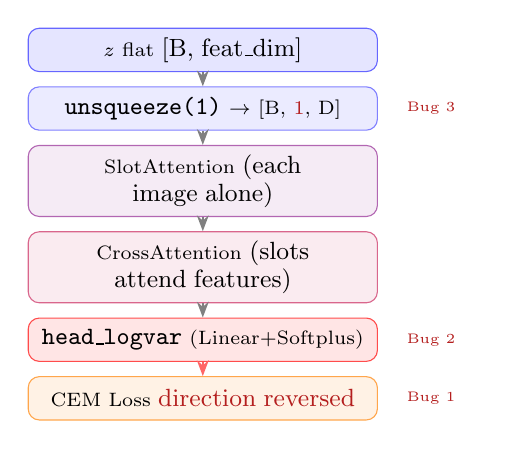
\begin{tikzpicture}[
    arr/.style={-{Stealth[length=2mm]}, thick, gray},
    badarr/.style={-{Stealth[length=2mm]}, thick, red!60},
    every node/.style={rectangle, rounded corners, text width=4.2cm,
                       minimum height=0.55cm, align=center, font=\scriptsize},
]
\node[draw=blue!60, fill=blue!10] (inp) {$z$ flat \small[B, feat\_dim]};
\node[draw=blue!50, fill=blue!8, below=0.18cm of inp] (uns) {\code{unsqueeze(1)} $\to$ [B, \bad{1}, D]};
\node[draw=violet!60, fill=violet!8, below=0.18cm of uns] (sa) {SlotAttention \small(each image alone)};
\node[draw=purple!60, fill=purple!8, below=0.18cm of sa] (ca) {CrossAttention \small(slots attend features)};
\node[draw=red!70, fill=red!10, below=0.18cm of ca] (hv) {\code{head\_logvar} (Linear+Softplus)};
\node[draw=orange!70, fill=orange!10, below=0.18cm of hv] (loss) {CEM Loss \small \bad{direction reversed}};

\draw[arr] (inp) -- (uns);
\draw[arr] (uns) -- (sa);
\draw[arr] (sa) -- (ca);
\draw[arr] (ca) -- (hv);
\draw[badarr] (hv) -- (loss);

\node[draw=none, fill=none, right=0.05cm of uns, font=\tiny\color{red}, text width=1cm] {\bad{Bug 3}};
\node[draw=none, fill=none, right=0.05cm of hv, font=\tiny\color{red}, text width=1cm] {\bad{Bug 2}};
\node[draw=none, fill=none, right=0.05cm of loss, font=\tiny\color{red}, text width=1cm] {\bad{Bug 1}};
\end{tikzpicture}
\end{column}

\begin{column}{0.48\textwidth}
\textbf{\fix{cem-fixed SlotCrossAttentionCEM}}

\vspace{0.2cm}
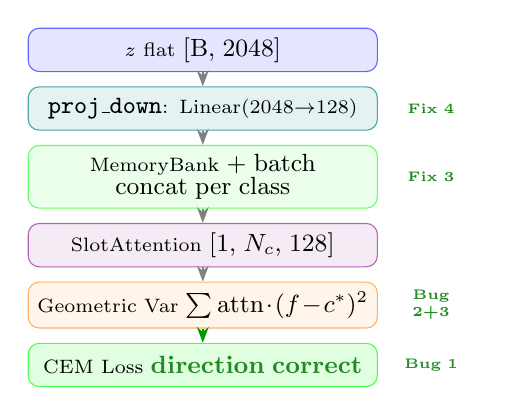
\begin{tikzpicture}[
    arr/.style={-{Stealth[length=2mm]}, thick, gray},
    goodarr/.style={-{Stealth[length=2mm]}, thick, green!60!black},
    every node/.style={rectangle, rounded corners, text width=4.2cm,
                       minimum height=0.55cm, align=center, font=\scriptsize},
]
\node[draw=blue!60, fill=blue!10] (inp) {$z$ flat \small[B, 2048]};
\node[draw=teal!70, fill=teal!10, below=0.18cm of inp] (proj) {\code{proj\_down}: Linear(2048$\to$128)};
\node[draw=green!60, fill=green!8, below=0.18cm of proj] (bank) {MemoryBank \small + batch concat per class};
\node[draw=violet!60, fill=violet!8, below=0.18cm of bank] (sa) {SlotAttention \small[1, $N_c$, 128]};
\node[draw=orange!60, fill=orange!8, below=0.18cm of sa] (var) {Geometric Var \small $\sum\text{attn}\cdot(f-c^*)^2$};
\node[draw=green!70, fill=green!12, below=0.18cm of var] (loss) {CEM Loss \small \fix{direction correct}};

\draw[arr] (inp) -- (proj);
\draw[arr] (proj) -- (bank);
\draw[arr] (bank) -- (sa);
\draw[arr] (sa) -- (var);
\draw[goodarr] (var) -- (loss);

\node[draw=none, fill=none, right=0.05cm of proj, font=\tiny\color{goodgreen}, text width=1cm] {\fix{Fix 4}};
\node[draw=none, fill=none, right=0.05cm of bank, font=\tiny\color{goodgreen}, text width=1cm] {\fix{Fix 3}};
\node[draw=none, fill=none, right=0.05cm of var, font=\tiny\color{goodgreen}, text width=1cm] {\fix{Bug 2+3}};
\node[draw=none, fill=none, right=0.05cm of loss, font=\tiny\color{goodgreen}, text width=1cm] {\fix{Bug 1}};
\end{tikzpicture}
\end{column}
\end{columns}

\end{frame}

% ============================================================================
\begin{frame}{Bug 1: Loss Direction is Completely Reversed}

\begin{columns}[T]
\begin{column}{0.5\textwidth}
\textbf{\bad{Original formula:}}
\[ \mathcal{L} = \text{ReLU}\!\Big(\log(\theta) - \log(\bar{v} + \varepsilon)\Big) \]
\vspace{-0.1cm}
\begin{itemize}\small
    \item Positive when $\bar{v} < \theta$ (variance \textbf{below} threshold)
    \item Penalizes \textbf{low variance} $\Rightarrow$ drives variance \textbf{up}
    \item Encoder pushed to \textbf{spread} same-class features
    \item \bad{Opposite to CEM intent — helps the attacker}
\end{itemize}
\end{column}
\begin{column}{0.5\textwidth}
\textbf{\fix{cem-fixed formula:}}
\[ \mathcal{L} = \text{ReLU}\!\Big(\log(\bar{v} + \gamma) - \log(\theta)\Big) \]
\vspace{-0.1cm}
\begin{itemize}\small
    \item Positive when $\bar{v} > \theta$ (variance \textbf{above} threshold)
    \item Penalizes \textbf{high variance} $\Rightarrow$ drives variance \textbf{down}
    \item Encoder pushed to \textbf{compress} features into tight sub-clusters
    \item \fix{Gradient direction matches CEM defense goal}
\end{itemize}
\vspace{0.1cm}
{\small Threshold: $\theta = \texttt{var\_thr} \times \texttt{reg\_str}^2 + \gamma$, $\;\gamma{=}0.01$}
\end{column}
\end{columns}

\vspace{0.15cm}
\begin{alertblock}{Impact}
\small With the original formula, increasing \texttt{lambd} would \textit{actively degrade} privacy. Every step was working \textbf{against} the defense.
\end{alertblock}

\end{frame}

% ============================================================================
\begin{frame}{Bug 2: Variance Predicted by Network, Not Computed Geometrically}

\begin{columns}[T]
\begin{column}{0.5\textwidth}
\textbf{\bad{Original: neural network predicts variance}}

\vspace{0.2cm}
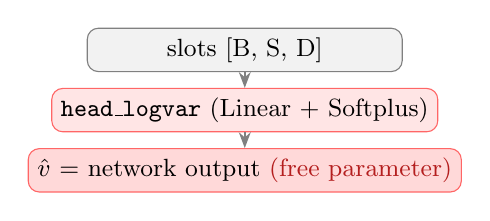
\begin{tikzpicture}[
    block/.style={rectangle, rounded corners, draw=gray, fill=gray!10,
                  minimum width=4cm, minimum height=0.5cm, align=center, font=\small},
    arr/.style={-{Stealth[length=2mm]}, thick, gray}
]
\node[block] (slots) {slots [B, S, D]};
\node[block, below=0.2cm of slots, fill=red!10, draw=red!60] (hv) {\code{head\_logvar} (Linear + Softplus)};
\node[block, below=0.2cm of hv, fill=red!15, draw=red!60] (var) {$\hat{v}$ = network output \bad{(free parameter)}};
\draw[arr] (slots) -- (hv);
\draw[arr] (hv) -- (var);
\end{tikzpicture}

\vspace{0.2cm}
\begin{itemize}
    \item \code{head\_logvar} has its own learnable weights
    \item Network can satisfy loss by \textbf{adjusting its own weights}, not the encoder
    \item CEM pressure is \textbf{absorbed by the prediction head}
    \item Encoder features are \textbf{unconstrained} — no defense effect
\end{itemize}
\end{column}
\begin{column}{0.5\textwidth}
\textbf{\fix{cem-fixed: geometric computation}}

\vspace{0.2cm}
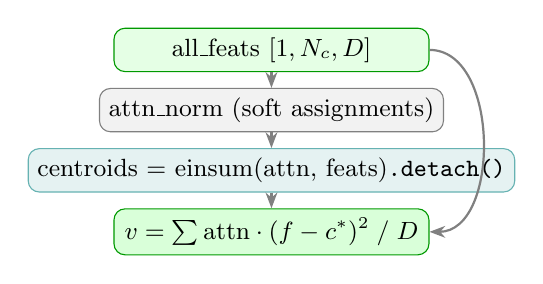
\begin{tikzpicture}[
    block/.style={rectangle, rounded corners, draw=gray, fill=gray!10,
                  minimum width=4cm, minimum height=0.5cm, align=center, font=\small},
    arr/.style={-{Stealth[length=2mm]}, thick, gray}
]
\node[block, fill=green!10, draw=green!60!black] (feats) {all\_feats $[1, N_c, D]$};
\node[block, below=0.2cm of feats] (attn) {attn\_norm (soft assignments)};
\node[block, below=0.2cm of attn, fill=teal!10, draw=teal!60] (cent) {centroids $=$ einsum(attn, feats)\code{.detach()}};
\node[block, below=0.2cm of cent, fill=green!15, draw=green!60!black] (var) {$v = \sum \text{attn} \cdot (f - c^*)^2 \;/\; D$};
\draw[arr] (feats) -- (attn);
\draw[arr] (attn) -- (cent);
\draw[arr] (cent) -- (var);
\draw[arr] (feats.east) to[out=0,in=0] (var.east);
\end{tikzpicture}

\vspace{0.2cm}
\begin{itemize}
    \item Variance = \textbf{actual Euclidean distance} from features to centroids
    \item No learnable parameters involved in variance computation
    \item Gradients go \textbf{directly to encoder features}
\end{itemize}
\end{column}
\end{columns}

\end{frame}

% ============================================================================
\begin{frame}{Bug 3: Slot Attention Clusters Within One Image, Not Across Samples}

\textbf{The largest semantic error.} CEM needs cross-sample clustering; the original version does intra-sample operation.

\vspace{0.2cm}
\begin{columns}[T]
\begin{column}{0.5\textwidth}
\textbf{\bad{Original: each image is processed alone}}

\vspace{0.1cm}
\begin{center}
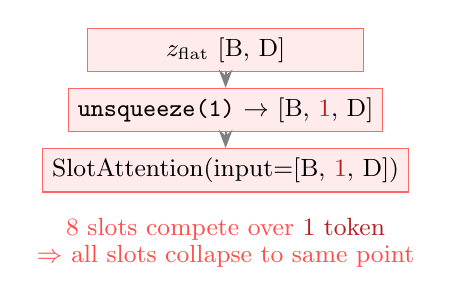
\begin{tikzpicture}[scale=0.85,
    block/.style={rectangle, draw=red!60, fill=red!8, minimum width=3.5cm,
                  minimum height=0.5cm, align=center, font=\small}
]
\node[block] (z) {$z_{\text{flat}}$ [B, D]};
\node[block, below=0.2cm of z] (uns) {\code{unsqueeze(1)} $\to$ [B, \bad{1}, D]};
\node[block, below=0.2cm of uns] (sa) {SlotAttention(input=[B, \bad{1}, D])};
\node[font=\small, below=0.2cm of sa, text=red!70] {8 slots compete over \bad{1 token}};
\node[font=\small, below=0.05cm of sa, yshift=-0.5cm, text=red!70] {$\Rightarrow$ all slots collapse to same point};
\draw[-{Stealth}, thick, gray] (z) -- (uns);
\draw[-{Stealth}, thick, gray] (uns) -- (sa);
\end{tikzpicture}
\end{center}
\end{column}
\begin{column}{0.5\textwidth}
\textbf{\fix{cem-fixed: cluster same-class samples together}}

\vspace{0.1cm}
\begin{center}
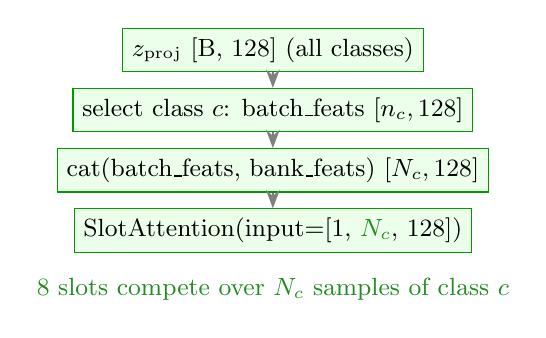
\begin{tikzpicture}[scale=0.85,
    block/.style={rectangle, draw=green!60!black, fill=green!8, minimum width=3.8cm,
                  minimum height=0.5cm, align=center, font=\small}
]
\node[block] (z) {$z_{\text{proj}}$ [B, 128] (all classes)};
\node[block, below=0.2cm of z] (sel) {select class $c$: batch\_feats $[n_c, 128]$};
\node[block, below=0.2cm of sel] (cat) {cat(batch\_feats, bank\_feats) $[N_c, 128]$};
\node[block, below=0.2cm of cat] (sa) {SlotAttention(input=[1, \good{$N_c$}, 128])};
\node[font=\small, below=0.2cm of sa, text=goodgreen] {8 slots compete over $N_c$ \good{samples of class $c$}};
\draw[-{Stealth}, thick, gray] (z) -- (sel);
\draw[-{Stealth}, thick, gray] (sel) -- (cat);
\draw[-{Stealth}, thick, gray] (cat) -- (sa);
\end{tikzpicture}
\end{center}
\end{column}
\end{columns}

\vspace{0.2cm}
\small
\textbf{Why it matters:} CEM's goal is to find \textit{sub-groups within each class}. This requires observing multiple samples of the same class simultaneously. With a single token as input, Slot Attention has nothing to cluster — 8 slots simply mirror the one input token.

\end{frame}

% ============================================================================
\begin{frame}{Engineering Fix 1: FeatureMemoryBank}

\small\textbf{Problem}: After fixing Bug 3, each class appears in a batch of 64 only $\sim$1--2 times (530 classes). $N_c < 2$ $\Rightarrow$ class \textbf{skipped entirely}.

\vspace{0.1cm}
\begin{columns}[T]
\begin{column}{0.52\textwidth}
\textbf{FeatureMemoryBank design:}

\vspace{0.05cm}
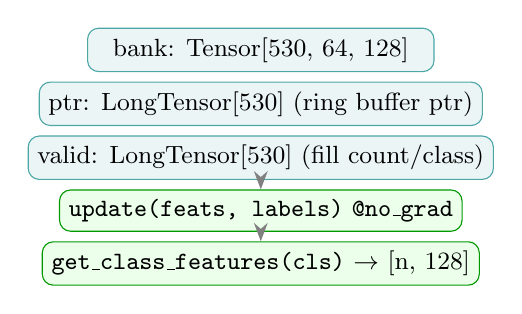
\begin{tikzpicture}[scale=0.82,
    block/.style={rectangle, rounded corners, draw=teal!70, fill=teal!8,
                  minimum width=4.4cm, minimum height=0.45cm, align=center, font=\small}
]
\node[block] (b1) {bank: Tensor[530, 64, 128]};
\node[block, below=0.12cm of b1] (b2) {ptr: LongTensor[530] \small (ring buffer ptr)};
\node[block, below=0.12cm of b2] (b3) {valid: LongTensor[530] \small (fill count/class)};
\node[block, below=0.12cm of b3, fill=green!8, draw=green!60!black] (upd) {\code{update(feats, labels)} \small\code{@no\_grad}};
\node[block, below=0.12cm of upd, fill=green!8, draw=green!60!black] (get) {\code{get\_class\_features(cls)} $\to$ [n, 128]};
\draw[-{Stealth}, thick, gray] (b3) -- (upd);
\draw[-{Stealth}, thick, gray] (upd) -- (get);
\end{tikzpicture}
\end{column}
\begin{column}{0.45\textwidth}
\textbf{How it feeds SlotAttention:}

\vspace{0.05cm}
\small
\begin{enumerate}
    \item Batch feats written to bank (\code{no\_grad})
    \item Class $c$: read up to 64 historical feats
    \item \code{cat([batch\_feats, bank\_feats])}
    \item SA receives $N_c = n_{\text{batch}} + n_{\text{bank}} \gg 2$
\end{enumerate}

\vspace{0.15cm}
\textbf{Key properties:}
\begin{itemize}
    \item bank feats: \textbf{no gradient} (history)
    \item batch feats: \textbf{has gradient} (drives encoder)
    \item Non-\code{Module} $\Rightarrow$ must override \code{.to(device)}
\end{itemize}
\end{column}
\end{columns}

\end{frame}

% ============================================================================
\begin{frame}{Engineering Fix 2: proj\_down for High-Dimensional Features}

\begin{block}{Problem}
\small FaceScrub encoder: $z=[B,8,16,16]$ $\xrightarrow{\text{flatten}}$ $[B,2048]$. SlotAttention directly on 2048-dim $\Rightarrow$ enormous parameter cost.
\end{block}

\vspace{0.1cm}
\begin{columns}[T]
\begin{column}{0.48\textwidth}
\textbf{Without proj\_down:}
\vspace{0.1cm}
\begin{center}
\small
\begin{tabular}{lrr}
\toprule
Layer & Size & Params \\
\midrule
\code{to\_q} & $2048 \times 2048$ & 4.2M \\
\code{to\_k} & $2048 \times 2048$ & 4.2M \\
\code{to\_v} & $2048 \times 2048$ & 4.2M \\
GRU & $2048 \times 2048$ & \warn{16.8M} \\
MLP & $2048 \times 4096$ & \warn{8.4M} \\
\midrule
\textbf{Total} & & \bad{$>$ 100M} \\
\bottomrule
\end{tabular}
\end{center}
\end{column}
\begin{column}{0.48\textwidth}
\textbf{With proj\_down (slot\_dim=128):}
\vspace{0.1cm}
\begin{center}
\small
\begin{tabular}{lrr}
\toprule
Layer & Size & Params \\
\midrule
\code{proj\_down} & $2048 \times 128$ & 0.26M \\
\code{to\_q} & $128 \times 128$ & 16K \\
\code{to\_k} & $128 \times 128$ & 16K \\
\code{to\_v} & $128 \times 128$ & 16K \\
GRU & $128 \times 128$ & 66K \\
MLP & $128 \times 256$ & 33K \\
\midrule
\textbf{Total} & & \good{$\sim$0.5M} \\
\bottomrule
\end{tabular}
\end{center}
\end{column}
\end{columns}

\vspace{0.1cm}
\footnotesize
\textbf{Gradient still flows}: $\nabla_{\theta_f} = \frac{\partial \mathcal{L}}{\partial z_{\text{proj}}} \cdot \frac{\partial z_{\text{proj}}}{\partial z_{\text{flat}}} \cdot \frac{\partial z_{\text{flat}}}{\partial \theta_f}$. \code{proj\_down} is differentiable — all 2048 dims receive CEM gradients.

\end{frame}

% ============================================================================
\begin{frame}{Engineering Fix 3: Detach Centroids to Close Gradient Shortcut}

\begin{columns}[T]
\begin{column}{0.50\textwidth}
\textbf{The shortcut (without \code{.detach()}):}

\vspace{0.2cm}
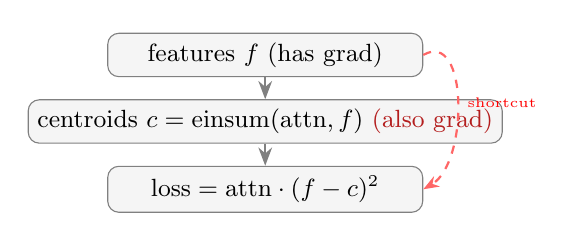
\begin{tikzpicture}[scale=0.72,
    block/.style={rectangle, rounded corners, draw=gray, fill=gray!8,
                  minimum width=4cm, minimum height=0.48cm, align=center, font=\small}
]
\node[block] (feats) {features $f$ (has grad)};
\node[block, below=0.28cm of feats] (cent) {centroids $c = \text{einsum}(\text{attn}, f)$ \bad{(also grad)}};
\node[block, below=0.28cm of cent] (diff) {$\text{loss} = \text{attn} \cdot (f - c)^2$};

\draw[-{Stealth}, thick, gray] (feats.south) -- (cent.north);
\draw[-{Stealth}, thick, gray] (cent.south) -- (diff.north);
\draw[-{Stealth[length=2mm]}, thick, red!60, dashed] (feats.east) to[out=30,in=30]
    node[right, font=\tiny, text=red, align=left] {shortcut} (diff.east);
\end{tikzpicture}

\vspace{0.2cm}
\small
\bad{Two gradient paths:}
\begin{enumerate}
    \item features move toward centroid \good{(correct)}
    \item centroid moves toward features \bad{(shortcut!)}
\end{enumerate}
Path 2 satisfies the loss with \textbf{zero encoder change}.
\end{column}
\begin{column}{0.47\textwidth}
\textbf{With \code{.detach()} (cem-fixed):}

\vspace{0.15cm}
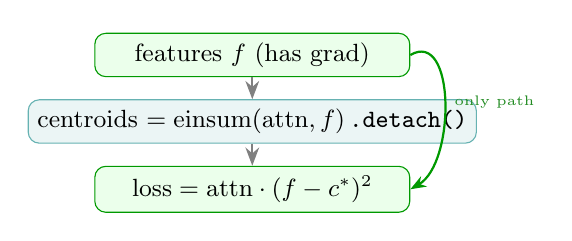
\begin{tikzpicture}[scale=0.72,
    block/.style={rectangle, rounded corners, draw=gray, fill=gray!8,
                  minimum width=4cm, minimum height=0.48cm, align=center, font=\small}
]
\node[block, fill=green!8, draw=green!60!black] (feats) {features $f$ (has grad)};
\node[block, below=0.28cm of feats, fill=teal!8, draw=teal!60] (cent) {centroids $= \text{einsum}(\text{attn},f)$\,\code{.detach()}};
\node[block, below=0.28cm of cent, fill=green!8, draw=green!60!black] (diff) {$\text{loss} = \text{attn} \cdot (f - c^*)^2$};

\draw[-{Stealth}, thick, gray] (feats.south) -- (cent.north);
\draw[-{Stealth}, thick, gray] (cent.south) -- (diff.north);
\draw[-{Stealth[length=2mm]}, thick, green!60!black] (feats.east) to[out=30,in=30]
    node[right, font=\tiny, text=goodgreen, align=left] {only path} (diff.east);
\end{tikzpicture}

\vspace{0.15cm}
\footnotesize
\fix{One gradient path only:} Features must truly approach the fixed centroid. Encoder cannot ``cheat'' by moving the reference point.
\end{column}
\end{columns}

\end{frame}

% ============================================================================
\begin{frame}{Engineering Fix 4: Deterministic Inference}

\begin{columns}[T]
\begin{column}{0.52\textwidth}
\textbf{\bad{Original: always random slot initialization}}

\vspace{0.1cm}
\small
\begin{center}
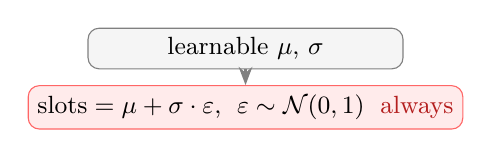
\begin{tikzpicture}[scale=0.9,
    block/.style={rectangle, rounded corners, draw=gray, fill=gray!8,
                  minimum width=4cm, minimum height=0.48cm, align=center, font=\small}
]
\node[block] (mu) {learnable $\mu$, $\sigma$};
\node[block, below=0.2cm of mu, fill=red!8, draw=red!60] (rnd) {$\text{slots} = \mu + \sigma \cdot \varepsilon$, $\;\varepsilon \sim \mathcal{N}(0,1)$ \;\bad{always}};
\draw[-{Stealth}, thick, gray] (mu) -- (rnd);
\end{tikzpicture}
\end{center}

\vspace{0.2cm}
\begin{itemize}
    \item During MIA evaluation, each forward pass gives \textbf{different attention distributions}
    \item CEM statistics fluctuate across evaluation runs
    \item Results are \textbf{not reproducible}; fair comparison is impossible
\end{itemize}
\end{column}
\begin{column}{0.45\textwidth}
\textbf{\fix{cem-fixed: train/eval split}}

\vspace{0.1cm}
\small
\begin{center}
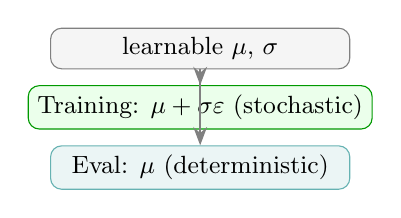
\begin{tikzpicture}[scale=0.9,
    block/.style={rectangle, rounded corners, draw=gray, fill=gray!8,
                  minimum width=3.8cm, minimum height=0.48cm, align=center, font=\small}
]
\node[block] (mu) {learnable $\mu$, $\sigma$};
\node[block, below=0.2cm of mu, fill=green!8, draw=green!60!black] (tr) {Training: $\mu + \sigma \varepsilon$ \small (stochastic)};
\node[block, below=0.2cm of tr, fill=teal!8, draw=teal!60] (ev) {Eval: $\mu$ (deterministic)};
\draw[-{Stealth}, thick, gray] (mu) -- (tr);
\draw[-{Stealth}, thick, gray] (mu) -- (ev);
\end{tikzpicture}
\end{center}

\vspace{0.2cm}
\begin{itemize}
    \item Training: stochastic init preserves exploration, prevents slot collapse
    \item Inference: deterministic init gives \textbf{identical output} for same features
    \item MIA evaluation results are \fix{fully reproducible}
\end{itemize}
\end{column}
\end{columns}

\end{frame}

% ============================================================================
\begin{frame}{Complete Bug \& Fix Summary}

\begin{center}
\footnotesize\setlength{\tabcolsep}{4pt}
\renewcommand{\arraystretch}{1.1}
\begin{tabular}{p{0.4cm}p{2.8cm}p{4.6cm}p{4.2cm}}
\toprule
& \textbf{Issue} & \textbf{Original Behavior} & \textbf{cem-fixed} \\
\midrule
\rowcolor{red!6}
\bad{B1} & Loss direction & $\text{ReLU}(\log\theta - \log v)$: penalizes low var; \textbf{drives features apart} & $\text{ReLU}(\log v - \log\theta)$: penalizes high var; \good{drives features together} \\
\rowcolor{red!6}
\bad{B2} & Variance source & Network-predicted (\code{head\_logvar}); pressure absorbed by head, \textbf{encoder unconstrained} & Geometric $\sum\text{attn}(f-c^*)^2$; \good{gradient direct to encoder} \\
\rowcolor{red!6}
\bad{B3} & Clustering object & Each image alone $[B,1,D]$; 8 slots on 1 token $=$ \textbf{meaningless} & Same-class samples $[1,N_c,D]$; \good{cross-sample sub-groups} \\
\midrule
\rowcolor{green!5}
\fix{F1} & Sample shortage & --- & \code{FeatureMemoryBank}: 64 feats/class; \good{every class has signal} \\
\rowcolor{green!5}
\fix{F2} & High-dim cost & SlotAttn in 2048-dim: \bad{100M+ params} & \code{proj\_down}(2048$\to$128): \good{$\sim$0.5M, grad preserved} \\
\rowcolor{green!5}
\fix{F3} & Centroid shortcut & No detach: centroid chases features & \code{.detach()}: \good{features must genuinely converge} \\
\rowcolor{green!5}
\fix{F4} & Non-determinism & Always stochastic slots & \good{Deterministic eval; stochastic train} \\
\bottomrule
\end{tabular}
\end{center}

\end{frame}

% ============================================================================
\begin{frame}{Why cem-fixed Should Outperform the Original Version}

\begin{columns}[T]
\begin{column}{0.55\textwidth}
\textbf{End-to-end signal path (cem-fixed):}

\vspace{0.1cm}
\begin{center}
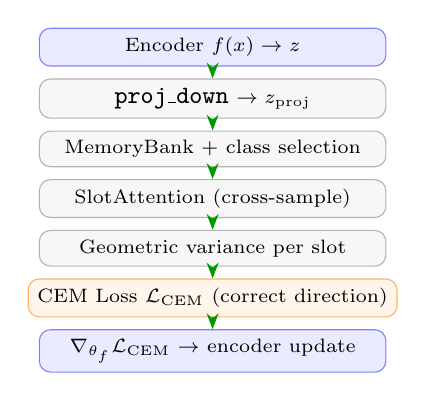
\begin{tikzpicture}[scale=0.78,
    block/.style={rectangle, rounded corners, draw=gray!60, fill=gray!6,
                  minimum width=4.4cm, minimum height=0.44cm, align=center, font=\scriptsize},
    arr/.style={-{Stealth[length=2mm]}, thick, green!60!black}
]
\node[block, fill=blue!8, draw=blue!50] (enc) {Encoder $f(x) \to z$};
\node[block, below=0.15cm of enc] (proj) {\code{proj\_down} $\to z_{\text{proj}}$};
\node[block, below=0.15cm of proj] (bank) {MemoryBank $+$ class selection};
\node[block, below=0.15cm of bank] (sa) {SlotAttention (cross-sample)};
\node[block, below=0.15cm of sa] (var) {Geometric variance per slot};
\node[block, below=0.15cm of var, fill=orange!8, draw=orange!60] (loss) {CEM Loss $\mathcal{L}_{\text{CEM}}$ (correct direction)};
\node[block, below=0.15cm of loss, fill=blue!8, draw=blue!50] (grad) {$\nabla_{\theta_f} \mathcal{L}_{\text{CEM}}$ $\to$ encoder update};

\foreach \i/\j in {enc/proj, proj/bank, bank/sa, sa/var, var/loss, loss/grad}
    \draw[arr] (\i) -- (\j);
\end{tikzpicture}
\end{center}
\end{column}
\begin{column}{0.42\textwidth}
\textbf{What this achieves:}

\vspace{0.15cm}
\begin{itemize}\small
    \item CEM loss reflects \textbf{true geometric} feature distribution
    \item Gradient flows \textbf{unobstructed} to encoder via proj\_down
    \item Every class gets meaningful signal every step (MemoryBank)
    \item SlotAttention finds \textbf{real sub-clusters} in feature space
    \item Encoder \textbf{genuinely forced} to compress same-class features
\end{itemize}

\vspace{0.15cm}
\begin{block}{Defense Mechanism}
\small Tight sub-clusters $\Rightarrow$ attacker cannot distinguish identities $\Rightarrow$ blurry reconstruction $\Rightarrow$ \textbf{lower Inference SSIM}.
\end{block}
\end{column}
\end{columns}

\end{frame}

% ============================================================================
\begin{frame}{}
\vfill
\begin{center}
{\Huge\textbf{Thank You}}

\vspace{0.8cm}
{\large 3 fatal bugs fixed $+$ 4 engineering improvements\\
cem-fixed is ready to run on the server}

\vspace{0.6cm}
{\normalsize 20 experiments $\times$ $\sim$5h each on NV 5880 Ada (48GB)\\
Results in \texttt{run\_exp.sh} $\to$ \texttt{log/summary.csv}}
\end{center}
\vfill
\end{frame}

\end{document}
